\documentclass[11pt]{article}
\usepackage{fullpage}
\usepackage{algorithm}
\usepackage[noend]{algorithmic}
\usepackage{amsmath,amssymb,amsthm}
\usepackage{graphicx}
\graphicspath{{..../pdf/}{C:/Users/Owner/Desktop/Machine Learning/STAT_339-master/HW1/figures/}}


% These define new environments / formats for lemmas, definitions, running time, etc.
\newtheorem{lemma}{Lemma}
\newtheorem{definition}{Definition}
\newtheorem{notation}{Notation}
\newtheorem*{claim}{Claim}
\newtheorem{observation}{Observation}
\newtheorem{conjecture}[lemma]{Conjecture}
\newtheorem{theorem}[lemma]{Theorem}
\newtheorem{corollary}[lemma]{Corollary}
\newtheorem{proposition}[lemma]{Proposition}
\newtheorem*{rt}{Running Time}


% These define nice ways to format P and OPT (use \P or \opt)
\def\P{\ensuremath{\mathcal{P}}}
\def\opt{\ensuremath{\textsc{opt}}}


% enumerate uses a., b., c., ...
\renewcommand{\labelenumi}{\bf \alph{enumi}.}


%%% TODO: Fill out the appropriate homework number and your name below
%%%
%%%
% Changes the title box on the first page
\renewcommand\maketitle{
\begin{center}
\begin{tabular*}{6.44in}{l @{\extracolsep{\fill}}c r}
\bfseries  &  & \bfseries STAT 339 Spring 2020 \\
\bfseries&  & \bfseries  Homework 1 Solutions  \\
\bfseries   &   &  \bfseries Garrett Robins \\ 
\end{tabular*}
\end{center} }




%%
%%
%% THE REAL STUFF STARTS HERE
%%
%%
\begin{document}
\maketitle


%%% TODO: PLEASE PLACE THE HONOR CODE AND YOUR NAME/SIGNATURE HERE
\noindent Honor Code: I affirm I have adhered to the Honor Code in this assignment - Garrett Robins\\
\subsection*{Part  1: KNN Implementation}
% TODO: Your solution to P1 goes here. Other parts should be in separate documents.
Below is the graph I made for the KNN neighbors on the S1Train dataset. As you can see, the misclassification rate of the classifier was minimized on the validation set when K = 3. The misclassification rate of the training set was trivially minimized at K =1 and non-trivially minimized at K = 3. Thus, as the graph has a general upward trend for larger values of K, I believe K = 3 to be the value that minimizes misclassification rate. 
\begin{figure}[h!]
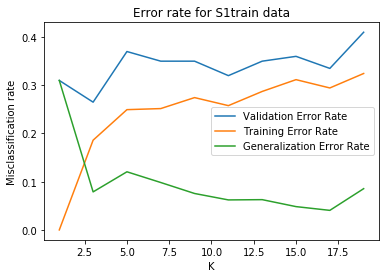
\includegraphics[width=210pt]{part1a_graph}
\centering
\end{figure} \\

Below is the graph I made for the KNN neighbors on the S2Train dataset. As you can see, the misclassification rate of the classifier was minimized on the validation set when K = 3. The misclassification rate of the training set was trivially minimized at K =1 and non-trivially minimized at K = 3. Thus, as the graph has a general upward trend for larger values of K, I believe K = 3 to be the value that minimizes misclassification rate. 
\begin{figure}[h!]
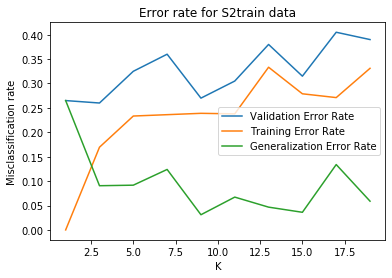
\includegraphics[width=210pt]{part1b_graph}
\centering
\end{figure} \\

From the sealed test sets, we should be able to find generalized performance for our K = 3 classifiers. In fact, when we train a KNN algorithm, with K = 3, with the training datasets, we see that the test datasets have these errors: \\
\begin{enumerate}
\item When the model is trained with S1train, the S1test dataset has a generalization error of {\bf .267}
\item When the model is trained with S2train, the S2test dataset has a generaization error of {\bf .295}
\end{enumerate} 
Although both of these data distributions had minimized classification error at K = 3, I don't know if I believe this to be true in general. It would seem that a more complex distribution would require more neighbors as reference points to minimize misclassification rate. To that end, it remains to be seen whether a more complex or simpler distribution leads to a higher K. \\ 
\subsection*{Part 2: KNN on Images}
Find below the graph of KNN neighbors on the image data given. Notice that this graph has minimized error for both the training and validation sets when K = 1. Although I am hesitant to use K = 1, as it has trivially 0 training error, the benefits seem to outweigh the costs and thus K = 1 is the optimal choice for K. (Note: the graph's title is wrong)   
\begin{figure}[h!]
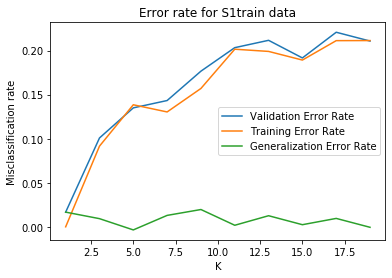
\includegraphics[width=300pt]{part2a_graph}
\centering
\end{figure} \\
When running a KNN algorithm trained on the training data on the test set, if we set K = 1 we get a {\bf.0137} misclassification rate. This is quite small and makes sense. In 28 dimensional data, you don't need many neighbors to confirm the type of image you're seeing. 
%% DON'T ERASE THIS LAST LINE
\end{document}
